%%%%%%%%%%%%%%%%%%%%%%%%%%%%%%%%%%%%%%%%%%%%%%
%
% Capítulo 1: Introducción
%
%%%%%%%%%%%%%%%%%%%%%%%%%%%%%%%%%%%%%%%%%%%%%%

\chapter{Introducción}

%%%%%%%%%%%%%%%%%%%%%%%%%%%%%%%%%%%%%%%%%%%%%%

\section{Antecedentes}
El análisis de patrones biométricos durante los últimos años ha tenido un gran número de aplicaciones: desde la comprobación de la identidad personal en aduanas hasta el reconocimiento de sonrisas en el momento de tomar una fotografía. El primer paso para llevarlo a cabo, es el reconocimiento de la cara en la imagen (técnicamente denominado determinación de la región de interés). Una vez disponemos de ella, se procede a la extracción de características de la imagen (almacenamiento en base de datos de una representación de la imagen). Ello se lleva a cabo a partir del reconocimiento de varios puntos característicos de la cara humana, entre los cuales podríamos destacar:

\begin{itemize}
	\item{Distancia entre ojos}
	\item{Ancho de la nariz}
	\item{Profundidad de las cuencas de los ojos}
	\item{Silueta marcada por los pómulos}
	\item{Ancho del mentón}
\end{itemize}


A partir de estos puntos característicos se crea una huella facial\footnote{Se ha considerado que es la mejor traducción del término inglés \textit{faceprint}} que es la representación numérica de los rasgos de un individuo.

%%%%%%%%%%%%%%%%%%%%%%%%%%%%%%%%%%%%%%%%%%%%%%

\subsection{Evolución de los métodos de reconocimiento}
La representación de las huellas faciales ha evolucionado con el tiempo hacia técnicas con menor probabilidad de fallo:
\begin{itemize}
	\item{Originalmente, la huella facial se obtenía a partir de una imagen en 2D comparada directamente con otra imagen 2D. Lamentablemente, este sistema requería que la expresión facial del evaluado fuese similar y el reconocimiento se veía muy influido por la iluminación ambiental. Este método se vendría a llamar PCA (de \textit{Principal Components Analysis}), y matemáticamente se basa en la extracción de eigenfaces (representaciones difusas de una matriz bidimensional). }
	\item{La evolución al sistema anterior fue el LDA (\textit{Linear Discriminant Analysis}) que ya se encarga de tomar la ubicación de los puntos característicos de la cara del individuo y calcular la distancia entre ellos. Tiene por mejoras la pérdida de sensitividad hacia la expresión facial y la menor dependencia de las condiciones de iluminación.}
	\item{El siguiente paso fue el uso de EBGM (del inglés \textit{ellastic bunch graph matching}) que consiste en, una vez tomadas las distancias entre puntos del método anterior, obtener los coeficientes de una transformada (normalmente Gabor) local a cada punto.}
	\item{El siguiente avance que se llevó a cabo fue la implementación de una malla tridimensional para el reconocimiento facial. Las ventajas son evidentes: reconocimiento en cualquier ángulo, independencia cuasi total de la iluminación y de la expresión facial. El principal incoveniente es la captura de la imagen original (tiene que obtenerse y componerse la imagen tridimensional).}
	\item{Actualmente los métodos empleados en los sistemas comerciales son mixtos. No se basan únicamente en las tecnologías previamente citadas, sino que además emplean técnicas para el reconocimiento de patrones dérmicos, obteniendo a la par que una \textit{faceprint}, una "huella dérmica" (\textit{skinprint}). Éste sistema, a partir de imágenes de alta resolución, detecta imperfecciones en la piel (poros, arrugas, etc.) hasta el punto de que es capaz de distinguir con una alta probabilidad hasta a gemelos idénticos.}
\end{itemize}

El software FaceIt® de \href{http://www.l1id.com/}{Identix} implementa la biometría dérmica previamente citada. Otras compañías que desarrollan software al respecto son \href{http://www.cognitec.com}{Cognitec}, \href{http://www.facerec.com/}{Aurora}, \href{http://www.id-arts.com/}{Id-arts} e \href{http://www.iwsinc.com}{ImageWare}.

%%%%%%%%%%%%%%%%%%%%%%%%%%%%%%%%%%%%

\section {Objetivos}
El objetivo de este proyecto es implementar un sistema de reconocimiento biométrico a partir del reconocimiento de patrones faciales. Mediante este, se implementará un sistema de control de accesos (Reloj de fichajes) para demostrar su correcto funcionamiento. Esta es una aplicación de ``relativa'' sencillez pero que muestra una de las utilidades que puede dar este sistema. 

Como subobjetivos podríamos mentar:
\begin{itemize}
	\item{Open Source: Todos los componentes empleados deben de tener disponible su código fuente.}
	\item{Establecer un esquema de BBDD ``genérico'' reaprovechable para la captura de otros rasgos biométricos (voz, iris, etc.). }
	\item{Modularidad: Con objeto de poder aislar mejor los problemas que pueda dar un componente y la reutilización de código se encapsulará este en clases que doten de la mayor independencia posible de otros componentes. }
	\item{Extensibilidad: Implementación bajo herramientas que faciliten añadir nuevas funcionalidades y mejorar las existentes. }
	\item{Inteligibilidad y documentación de código: Documentación de código para todas las partes que sea posible y uso de nombres de variables explícitos.}
\end{itemize}

%%%%%%%%%%%%%%%%%%%%%%%%%%%%%%%%%%%%

\subsection{Motivación y justificación}
La motivación y justificación del proyecto se basan en los siguientes puntos:
\begin{itemize}
	\item{\textbf{Reducción de costes}:} El equipamiento necesario por parte del usuario es inexistente (en el caso del reloj de fichajes, la tarjeta de identificación). Por parte del propietario, el equipamiento es muy económico (en el mismo caso,sería suficiente con una cámara y un equipo informático doméstico).
	\item{\textbf{Facilidad de uso}:} Debido al reconocimiento a partir de una parte normalmente a la vista como es la cara la identificación del individuo es sencilla.
\end{itemize}

%%%%%%%%%%%%%%%%%%%%%%%%%%%%%%%%%%%%

\subsection{Alcance}
La aplicación realizada no debería, emplearse en entornos críticos en cuanto a identificación de personal. Se debe tener en cuenta que el reconocimiento facial mediante el equipamiento que va a ser empleado es una técnica muy susceptible a posibles falsificaciones debido a los siguientes factores:
\begin{itemize}
	\item{\textbf{Autenticación a partir de imagen}:} Se podría dar como válida una fotografía impresa en lugar de la cara del individuo a identificar, dando lugar a falsos negativos tanto en la detección de rostros como en el reconocimiento del individuo.
	\item{\textbf{Oclusión/ocultación de rasgos faciales}:} Las bufandas, gafas de sol... así como la simple ocultación mediante las manos pueden reducir considerablemente el área facial a partir de la cual reconocer al individuo, propiciando así los falsos negativos en la detección de rostros.
	\item{\textbf{Variabilidad de rasgos faciales}:} Los accidentes, las operaciones estomatológicas (extracciones dentales, implantes, etc), la cirugía plástica, etc. pueden llevar a cabo modificaciones en los rasgos de un individuo, y por tanto dar falsos negativos en el reconocimiento de éste.
\end{itemize}

Como se ha comentado anteriormente, se busca construir un sistema basado en la modularidad (separación de funcionalidades en capas) y la extensibilidad (facilitar la adición de nuevas funcionalidades y mejora de los algoritmos). En el diseño se han considerado necesarias dos bases de datos y tres aplicaciones para cumplir el objetivo propuesto. Esto dota de mayor flexibilidad a la hora de implantar el sistema: número de puestos de captura, centralización, distribución, etc.

%%%%%%%%%%%%%%%%%%%%%%%%%%%%%%%%%%%%

\section{Software empleado}

Se ha empleado el siguiente software (cuya licencia se especifica también a continuación) para la implementación del proyecto. En los casos en los que se emplea el símbolo \textgreater (mayor que) es debido a que se han ido aplicando actualizaciones y parches de seguridad sobre dicho software durante el desarrollo del proyecto y la versión puede ser posterior a la indicada.
\begin{itemize}
	\item{\textbf{GNU/Linux} es el sistema operativo sobre el que todo se ha desarrollado y se sustenta. Salvo excepciones, la licencia de la gran mayoría de librerías y aplicaciones disponibles para éste es GPLv2 o superior\footnote{Actualmente sólo se ha testeado sobre la distribución Ubuntu.}.}
	\item{\textbf{Python} en su versión \textgreater2.6 como lenguaje de programación. La licencia aplicada sobre éste es PSFL (Python software foundation license), la cual es compatible con GPLv2 en esta versión del lenguaje.}
	\item{\textbf{GTK+ y Glade} en sus versiones \textgreater2.16 y \textgreater3.6 para diseñar el entorno gráfico. Los bindings de ésta librería para Python se encapsulan en la librería pygtk. La licencia de todos los componentes es GPLv2 o superior.}
	\item{\textbf{OpenCV} en su versión \textgreater1.0 como librería principal para la captura y la localización de la región de interés en la imagen. La licencia de dicho software es BSD, lo que permite que pueda ser empleada en proyectos GPL.}
\end{itemize}
Asímismo, para la realización de la documentación, gráficas, estadísticas y demás trabajo sobre imágenes se ha empleado el siguiente software:
\begin{itemize}
	\item{\textbf{Vim} como editor principal para la realización tanto de la documentación como de la gran mayoría del código fuente. Licencia CharityWare, compatible con GPLv2.}
	\item{\LaTeX{} para la documentación, concretamente en la distribución Texlive. Licencia GPLv2 o superior.}
	\item{\textbf{Doxygen} para la documentación del código. Licencia GPLv2 o superior. También se ha empleado el plugin \textit{Doxypy} que es un filtro para poder incluir tags de doxygen en los comentarios habituales de python y cuya licencia también es GPLv2.}
	\item{\textbf{Dia} para la elaboración de diagramas. Licencia GPLv2 o superior. Los diagramas se han exportado a \textit{tikz} que es una librería para generación de gráficos vectoriales en \LaTeX{}, licencia GPLv2. }
	\item{\textbf{Gnuplot} para la elaboración de gráficas estadísticas, exportadas a formato \LaTeX{}. La licencia NO es GPLv2, aunque sí que es Free Software y sólo se empleará para realizar gráficas.}
	\item{\textbf{Gimp} para el retoque de imágenes (principalmente pantallazos y similares). Licencia GPLv2 o superior.}
\end{itemize}

La gran mayoría (si no todo) el software empleado tiene una comunidad activa de colaboradores, soporte vía foros, manuales y documentación disponible en internet. 
	
%%%%%%%%%%%%%%%%%%%%%%%%%%%%%%%%%%%%

\subsection{Herramientas colaborativas y repositorios}
El sistema de control de versiones a emplear es GIT. GitHUB se ha considerado la mejor opción como comunidad para hospedar el proyecto por ofrece las siguientes funcionalidades:
\begin{itemize}
	\item{Repositorio para almacenar el proyecto}
	\item{Cuenta SSH desde las que hacer los Push y Pull de las revisiones}
	\item{Tablón para colgar anuncios en cuanto a la evolución del proyecto}
	\item{Interfaces web para editar código online, mostrar grafos de versionado, portapapeles de copiado web (pastebin), etc.}
\end{itemize}
Se ha decidido emplear una cuenta gratuíta en GitHUB, la cual ofrece hasta 300 Mb de almacenamiento, aun en las previsiones más extremas el tamaño del código no llega a ese nivel, y se creará un repositorio en dicha cuenta (el tiempo de creación es despreciable). Una de las múltiples vistas de este sitio aparece en la figura \ref{fig:interface_git}.  Los datos del usuario que se emplearán son los siguientes:
\begin{itemize}
	\item{\textbf{Nombre de usuario}: brunorro}
	\item{\textbf{Cuenta de correo}: br1.rdgz@gmail.com}
\end{itemize}

\begin{figure}
	\centering
	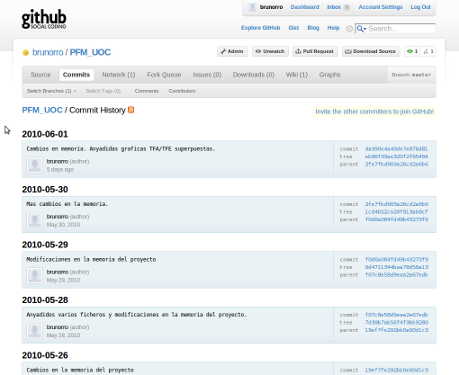
\includegraphics[width=11cm]{imagenes/interfazGit.png}
	\caption{Lista de commits de GitHub}
	\label{fig:interface_git}
\end{figure}

%%%%%%%%%%%%%%%%%%%%%%%%%%%%%%%%%%%%

\section{Planificación}
Se han estimado los siguientes puntos a los que imputar el tiempo empleado:
\begin{itemize}
	\item{\textbf{Diseño de la aplicación de gestión, captura y reconocimiento}: Tiempo durante el que se diseñarán los prototipos de las aplicaciones de las que consta el proyecto.}
	\item{\textbf{Diseño de la base de datos de gestión}: Tiempo empleado en diseñar la BD relacional que contendrá la información sobre el control de accesos.}
	\item{\textbf{Diseño de la base de datos de características}: Periodo durante el que se diseñará la BD relacional en la que se almacenará la representación facial de cada individuo.}
	\item{\textbf{Determinación de la representación en la BD}: Referente a la base de datos previa, durante este tiempo se investigará el método de almacenamiento para la representación facial.}
	\item{\textbf{Estadísticas}: Toma de datos y cálculos (gráficas) de eficiencia temporal, espacial y de funcionamiento.}
\end{itemize}
En la sección \ref{sec:cost_estimation} se definen los roles necesarios para llevar el proyecto, sus funciones y las estimaciones de tiempo de trabajo para cada uno de ellos. Tras la liberación se espera que los aspectos del desarrollo que no ha dado tiempo a finalizar (por falta de tiempo) se puedan pulir.
